\documentclass[notes]{beamer}       			% compila sia i frame che le note
%\documentclass{beamer}              			% compila solo i frame
%\documentclass[notes=only]{beamer}  	% compila solo le note

% ita language and encoding
\usepackage[utf8]{inputenc}
\usepackage[italian]{babel}

% graphics style
\usepackage{graphicx}
\usepackage{xcolor}
\usepackage{shadowtext}

%image paths
\graphicspath{{./Immagini/}}

% impostazioni base delle slide - tema, colori, caratteri, ... (deic.uab.es/~iblanes/beamer_gallery/)
\mode<presentation>
{
	\usetheme{CambridgeUS}      % or try Darmstadt, Madrid, Warsaw, ...
  	\usecolortheme{rose} 			% or try albatross, beaver, crane, orchid, rose ...
	\usefonttheme{structurebold} % or try structureitalicserif, structuresmallcapsserif
}

% settagio dati principali del file - titolo, autore, ...
\title[Università degli studi di Perugia]{L'esperimento AMS}
\subtitle{Review generale dell'apparato}
\author{Daniele Di Bari}
\institute[]{\small{Università degli studi di Perugia}\\ \small{Corso di laurea magistrale in fisica}}
\date[27 Aprile 2017]{\scriptsize{27 Aprile 2017}}
\subject{Rivelatori di Particelle}

% settaggio prima slide
\setbeamertemplate{title page}
{
	\shadowcolor{white!30!black}
	\vspace{-0.5cm}	
	
    \shadowtext{\textcolor{white}{\textbf{\footnotesize{The Alpha Magnetic Spectrometer}}}}
   
    \vspace{0.15cm}  	
    
   	\shadowtext{\textcolor{white}{\textbf{\LARGE \inserttitle}}}\par
      
   	\vspace{0.1cm}  

   	\shadowtext{\textcolor{white}{\emph{\large \insertsubtitle}}}\par
   	
   	\vspace{2.5cm}
	
	\titlepagetext{lightgray}{Il più grande rivelatore di particelle}\\
	\titlepagetext{lightgray}{nello spazio, montato sulla}\\
	\titlepagetext{lightgray}{Stazione Spaziale Internazionale}		
}
				
% colors
\definecolor{itemred}{RGB}{163,0,0}
\definecolor{itemblue}{RGB}{0,24,170}

% COMANDI
% Formato testo generico in titolpage
\newcommand\titlepagetext[2]{\textcolor{#1}{\footnotesize{\textit{{#2}}}}}

\begin{document}
% impostare una foto come sfondo del frame: 
\usebackgroundtemplate{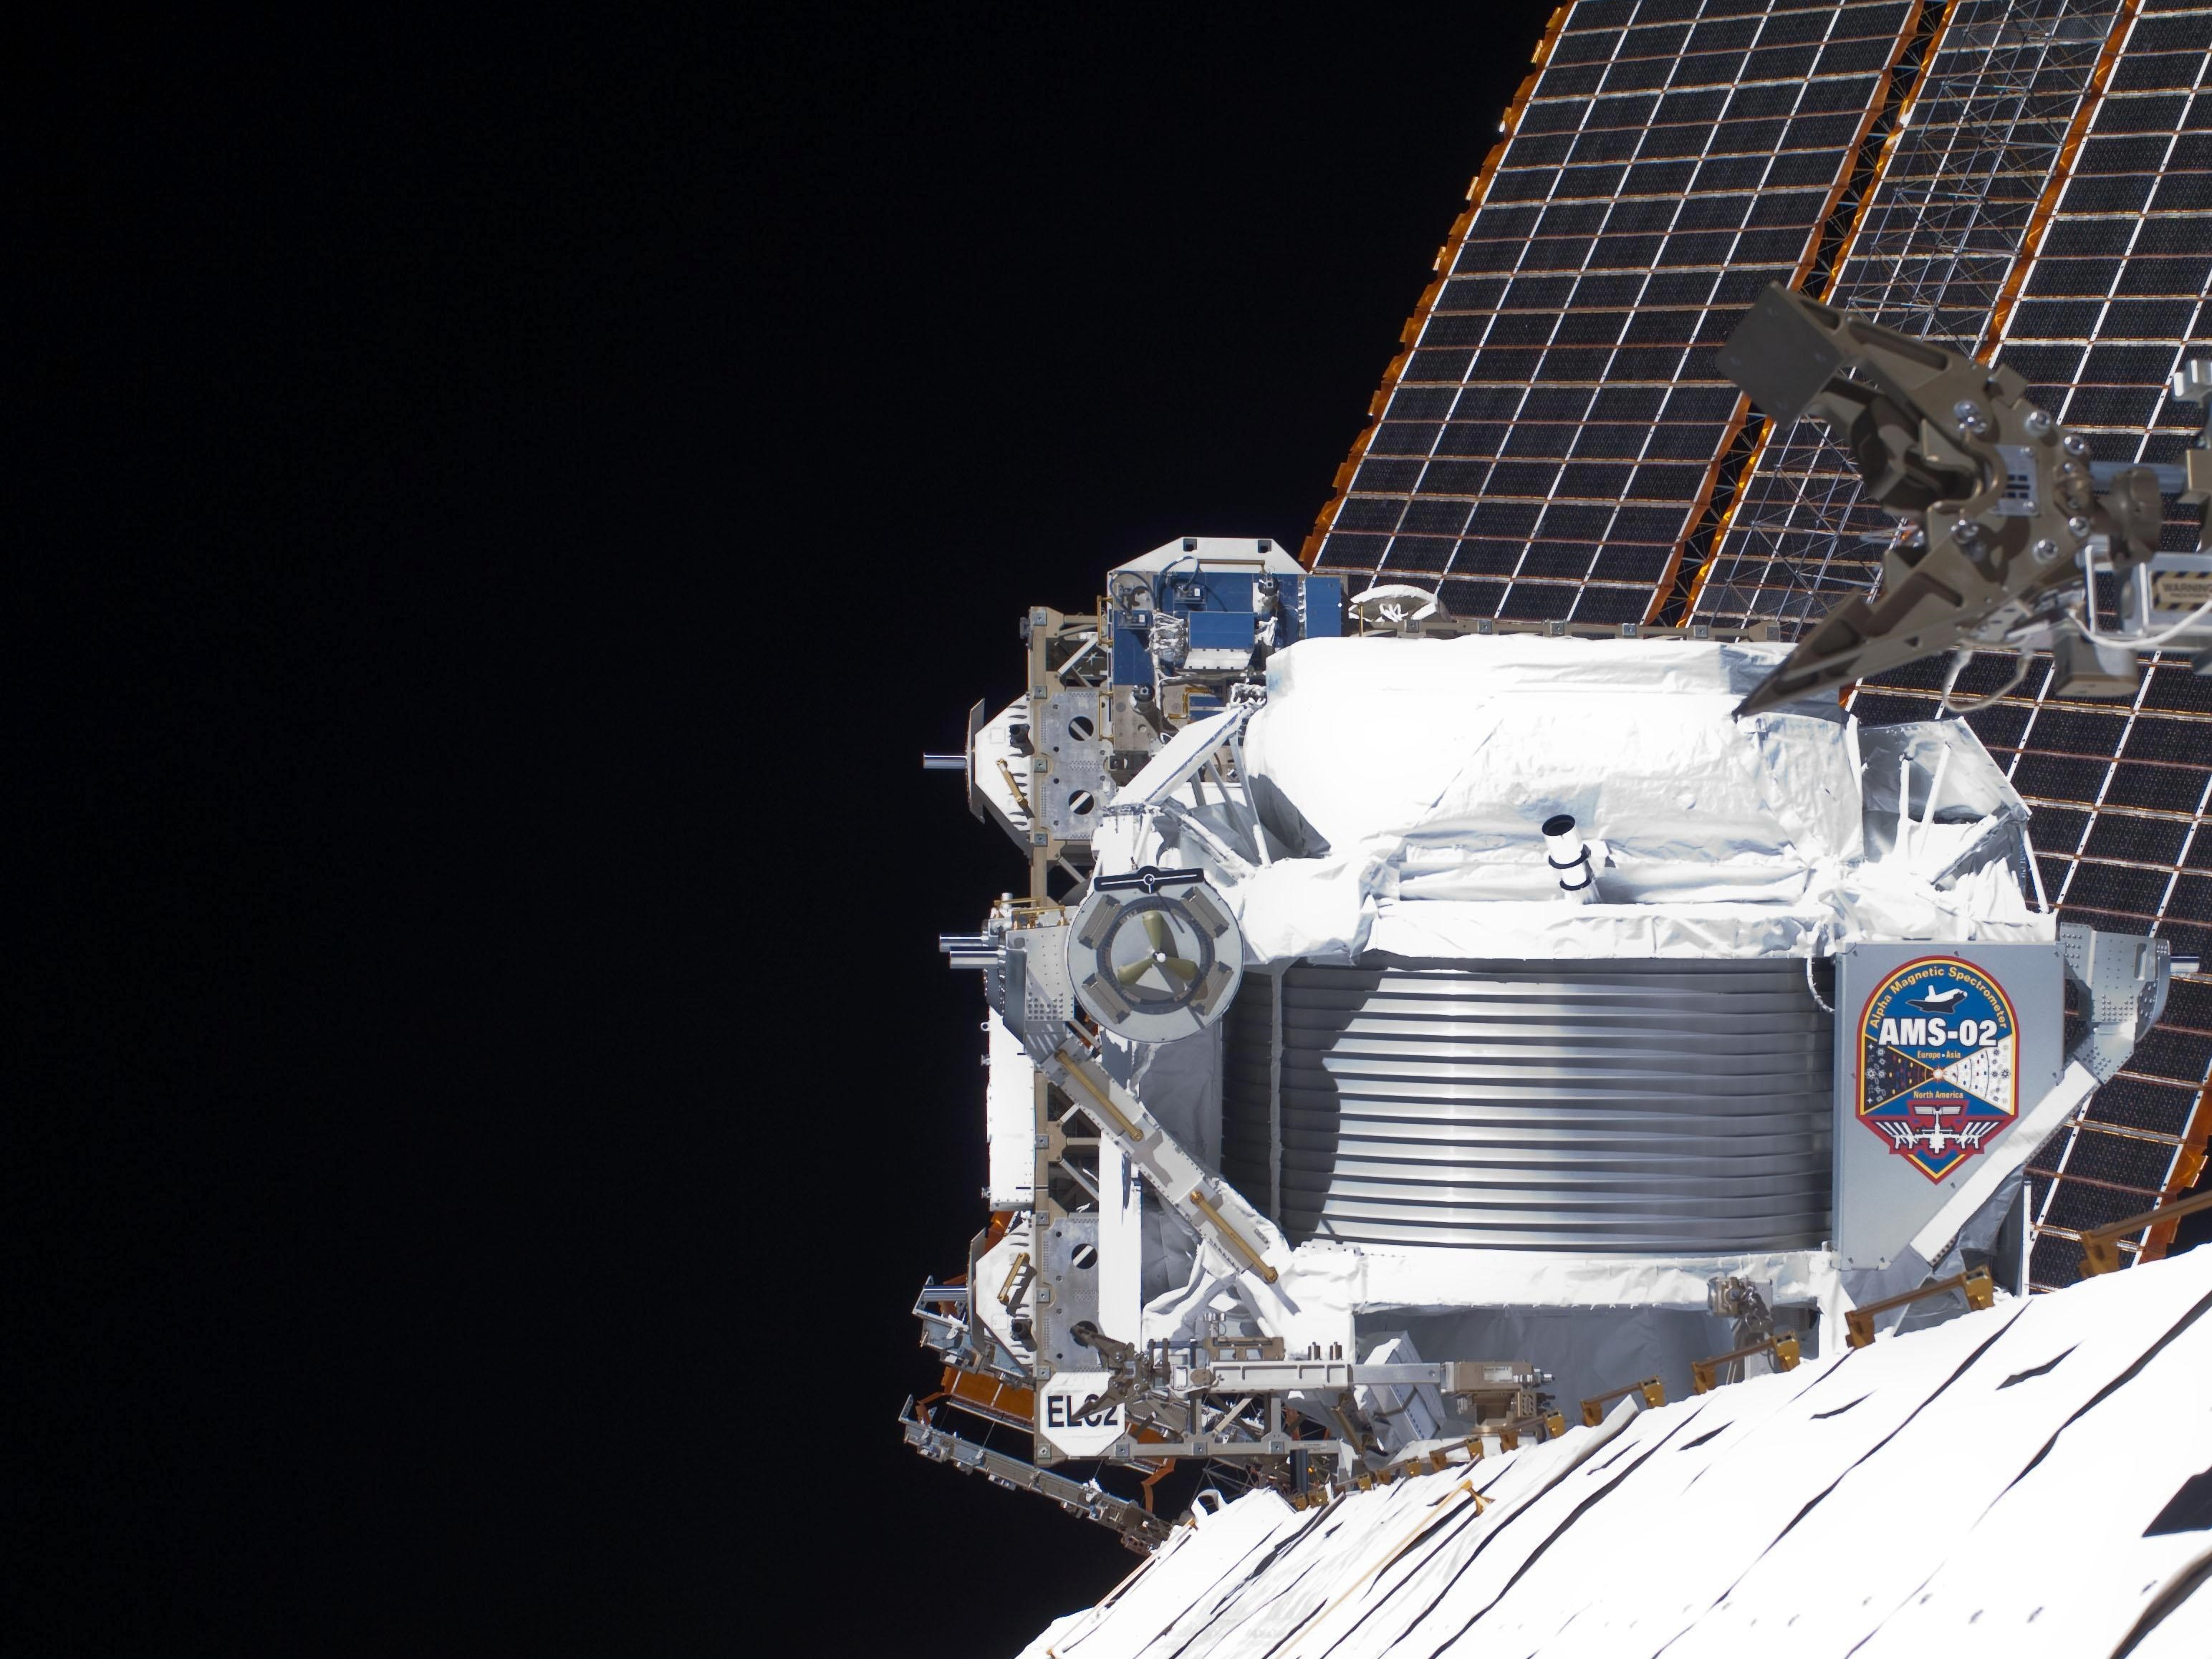
\includegraphics[height=\paperheight,keepaspectratio]{on_ISS-08_cutMIDDLEUP-3088.jpg}}	% possibili impostazioni per l'img: width=\paperwidth  --  height=\paperheight  --  keepaspectratio

\section{Corso di Rivelatori di Particelle}
\subsection{Presentazione dell'esperimento AMS}

\begin{frame}
	\titlepage
\end{frame}

\note{ 
   Salve, sono Gabriele di Bari e oggi parlerà della mia tesi che riguarda:\\
   Differential Evolution per reti neurali
}

\usebackgroundtemplate{}

\begin{frame}

\setbeamertemplate{background}{white}
\frametitle{Introduzione: Alpha Magnetic Spectrometer (AMS)}
Lo scopo dell'esperimento è quello di effettuare, per un periodo di lunga durata così da ottenere un'elevata statistica, delle misure molto accurate dello spettro di energia (per energie fino all'ordine dei TeV) dei raggi cosmici carichi primari direttamente nello spazio.

\vspace{0.25cm}
Obiettivi principali:
\begin{enumerate}
	\item Materia oscura
	\item Antimateria primordiale
	\item Abbondanze isotopiche dei raggi cosmici primari
\end{enumerate}

\end{frame}

\begin{frame}
	\frametitle{Detection of Charged Particles}
	\begin{itemize}
	\item	Che tipo ti particelle si vuole rivelare?
	\item	Qual'è la dimensione richiesta del rivelatore?
	\item	Quali caratteristiche delle particelle bisogna rivelare?
	\begin{itemize}
		\item[$\circ$]	Posizione - Traiettoria
		\item[$\circ$]	Tempo
		\item[$\circ$]	Numero
		\item[$\circ$]	Energia
		\item[$\circ$]	Quantità di moto
	\end{itemize}
	\item	Qual'è il massimo rate dei conteggi?
	\item	Qual'è la distribuzione temporale degli eventi?
	\item	Ed infine, ma non per ultimo, quanto costa? 
	\end{itemize}
\end{frame}

\begin{frame}
    \frametitle{Introduction}

\begin{itemize}
  \item Your introduction goes here!
  \item Use \texttt{itemize} to organize your main points.
\end{itemize}

\end{frame}

\note{Everything you want}

\begin{frame}
    \frametitle{Development}

    Lot of interesting things

\end{frame}

\note[itemize]{
\item point 1
\item point 2
}

\begin{frame}
    \frametitle{Development}

    Lot of interesting things

\end{frame}

\end{document}
